%%%%%%%%%%%%%%%%%%%%%%%%%%%%%%%%%%%%%%%%%%%%%%%%%%%%%%%%%%%%%%%%%%%%%%%
%% Document: Thesis for PhD at UC Riverside                          %%
%% Description: A comparative analysis of environment sensing in EDF %%
%% Author: Steven Ahrendt                                            %%
%%%%%%%%%%%%%%%%%%%%%%%%%%%%%%%%%%%%%%%%%%%%%%%%%%%%%%%%%%%%%%%%%%%%%%%
% RHODOPSIN FIGURES %
%%%%%%%%%%%%%%%%%%%%%
% Photosensory protein distribution in Fungi
\begin{figure}[hb]
  \centering
  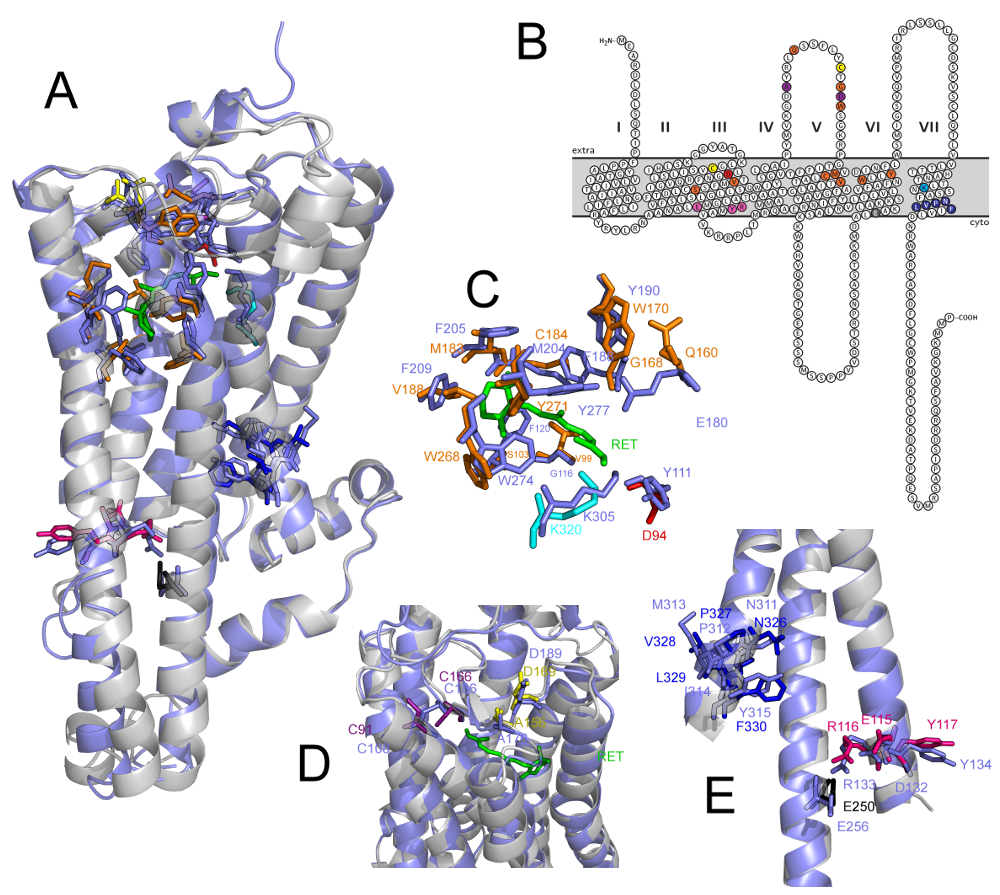
\includegraphics[width=4in]{./Chapter_RhodStruct/img/SpStructure.png}
  \caption[Structural details of the \textit{S. punctatus} chytriopsin homology model.]{Key \textit{S. punctatus} residues are colored according to function: orange (binding pocket residues), red (putative counterion), purple (disulfide bond), yellow (salt bridge), dark blue (NPxxY motif), and pink \& black (ion lock). Light purple functional and backbone residues belong to \textit{T. pacificus}, while grey backbone residues belong to \textit{S. punctatus}. The ideal position of the 11-\textit{cis}-retinal ligand, taken from the \textit{T. pacificus} crystal structure, is shown in green. A) C$\alpha$ backbone structural alignment of \textit{S. punctatus} homology model and \textit{T. pacificus} x-ray crystal structure, displayed in a cartoon representation, with key residues displayed as sticks. B) Topography plot of membrane spanning regions of \textit{S. punctatus} homology model. C) Detail of \textit{S. punctatus} binding pocket residues aligned with those of \textit{T. pacificus}. The lysine residue from \textit{S. punctatus} (cyan) is present in an optimal position to interact with the 11-\textit{cis}-retinal ligand (green), an aspect unique among the chytriopsins studied. The putative \textit{S. punctatus} counterion D94 (red) is also situated in an ideal position for photoisomerization. D) Detail of \textit{S. punctatus} disulfide bond (purple) and salt bridge (yellow) regions aligned with those of \textit{T. pacificus}. The view is from the top (extracellular side) of the protein, into the 11-\textit{cis}-retinal (green) binding pocket. E) Detail of \textit{S. punctatus} ERY and NPxxY regions aligned with those of \textit{T. pacificus}. In \textit{T. pacificus}, residues R133 and E256 (light purple) form a salt bridge in the inactive state to hold the structure in place, which is broken upon receptor activation. The corresponding \textit{S. punctatus} residues R116 (pink) and E250 (black) are in equivalent positions and presumably carry out the same function.}
  \label{fig:ChRhodS_SpStructure}
\end{figure}
